%!LW recipe=latexmk (XeLaTeX)
\documentclass[12pt,hyperref,a4paper,UTF8]{ctexart}
\usepackage{SJTUReport}
\usepackage{booktabs} % 三线表
\usepackage{amsmath}
\usepackage{amssymb} 

%%-------------------------------正文开始---------------------------%%
\begin{document}

% %-----------------------封面--------------------%%
\cover

%------------------摘要-------------%%
\newpage
\begin{abstract}

在此填写摘要内容

\end{abstract}
\newpage

\thispagestyle{empty} % 首页不显示页码

%%--------------------------目录页------------------------%%
\newpage
\tableofcontents

%%------------------------正文页从这里开始-------------------%
\newpage

%可选择这里也放一个标题
\begin{center}
   \title{ \Huge \textbf{{考虑异质用户的高速公路换电站运营MPC-RL分层协同优化}}}
\end{center}



\section{Introduction}
随着电动汽车在高速公路中长距离出行场景中的普及，沿线换电站的运营能力逐渐成为影响用户出行可靠性与系统运行效率的关键因素。相比传统充电方式，换电模式能够显著缩短车辆补能时间，但其运营过程同时受到用户到达需求、电池库存状态、站内充电过程以及电价变化等因素影响。特别是在高速公路场景中，用户行驶路径具有明显的方向性和连续性，不同车辆的初始 SOC 存在差异，导致其可达站点、可行换电路径以及对站内满电电池的占用情况均不相同。因此，高速公路换电站运营本质上是一个具有时空耦合、库存动态演化和不确定需求特征的序贯决策问题。

在实际运营中，系统中存在两类异质用户：预约用户和随机到达用户。预约用户通常提前给出出发时间、OD 路径和初始 SOC 信息，运营者需要在用户出行前对其换电站点进行合理分配，以提高服务确定性；随机用户的到达则具有更强的不确定性，运营者需要根据当前电池库存和未来需求预期决定是否服务。若仅基于当前满电电池数量进行局部决策，可能导致某些站点的满电电池被提前消耗，从而影响后续预约用户的服务可靠性；若过度保守地保留库存，又会降低随机用户服务量和系统收益。因此，如何在预约用户服务保障、随机用户灵活接纳以及电池充电调度之间进行协调，是高速公路换电网络运营中的核心问题。

针对上述问题，本文构建 MPC-RL 分层协同优化框架。换电站运营中存在两类性质不同但相互耦合的决策：一类是用户服务分配决策，包括预约用户路径指派和随机用户服务量决策；另一类是充电功率决策，即不同站点、不同 SOC 电池在不同时段的充电功率安排。本文采用模型预测控制（Model Predictive Control, MPC）处理用户服务分配问题，主要原因在于该问题包含 SOC 相关可达性、网络流平衡、满电电池可用性、预约用户优先级和库存非负性等硬约束，且可行动作集合会随 OD、初始 SOC、历史已出发车辆和站点库存动态变化。若直接采用 RL 进行用户指派，需要设计高维组合动作空间并处理大量动态 action masking，训练稳定性和可行性保障均较困难。相比之下，MPC 能够在滚动预测时域内显式刻画上述约束，并给出可解释、可执行的服务分配方案。

另一方面，充电功率决策虽然也可由 MPC 直接优化，但其影响具有明显的跨时段累积性：当前充电功率不仅决定当前充电成本，还会改变未来各站点不同 SOC 电池分布、满电电池供给能力和后续用户服务水平。由于充电功率动作维度相对固定，本文采用强化学习（Reinforcement Learning, RL）学习充电功率控制策略，使其能够在长期交互过程中根据需求、电价和库存状态自适应调整充电行为。如\autoref{fig:MPC-RL}所示，RL 层输出充电功率决策并影响电池状态转移，MPC 层在给定功率策略下优化预约用户和随机用户的服务分配。

进一步地，本文利用 RL critic 提供预测时域之外的长期价值信息，以缓解有限预测时域导致的末端效应。传统 MPC 通常通过设置固定终端库存下界避免时域末端过度消耗满电电池，但该方法只能粗略限制末端满电电池数量，难以区分不同站点、不同 SOC 电池在未来需求和电价环境下的长期价值。本文在 RL 训练过程中学习状态价值函数，并在每轮 MPC 求解前计算 critic 对终端库存的梯度，将其作为终端库存的长期边际价值系数。由此，RL 学到的长期价值被转化为 MPC 目标函数中的线性终端价值项，而无需将非线性神经网络直接嵌入优化模型。

因此，本文提出的 MPC-RL 框架并非将两类方法简单拼接，而是基于决策属性进行分层：MPC 负责处理强约束、组合结构明显且需要可解释性的用户服务分配问题；RL 负责学习具有长期影响的充电功率策略，并通过 critic 向 MPC 提供终端库存价值信息。二者通过电池库存状态、充电功率决策和终端价值项相互连接，从而在保证预约用户服务质量要求和运营约束可行性的同时，使有限时域 MPC 能够近似感知预测时域之外的长期影响。

本文其余部分安排如下：第 2 节介绍 MPC 优化模型，包括时域设置、变量定义、SOC-wise expanded network 建模方法以及数学规划模型；第 3 节介绍 RL formulation，包括马尔可夫决策过程的建立和所选 RL 算法；第 4 节和第 5 节分别预留实验分析和结论部分。

\begin{figure}[!htbp]
    \centering
    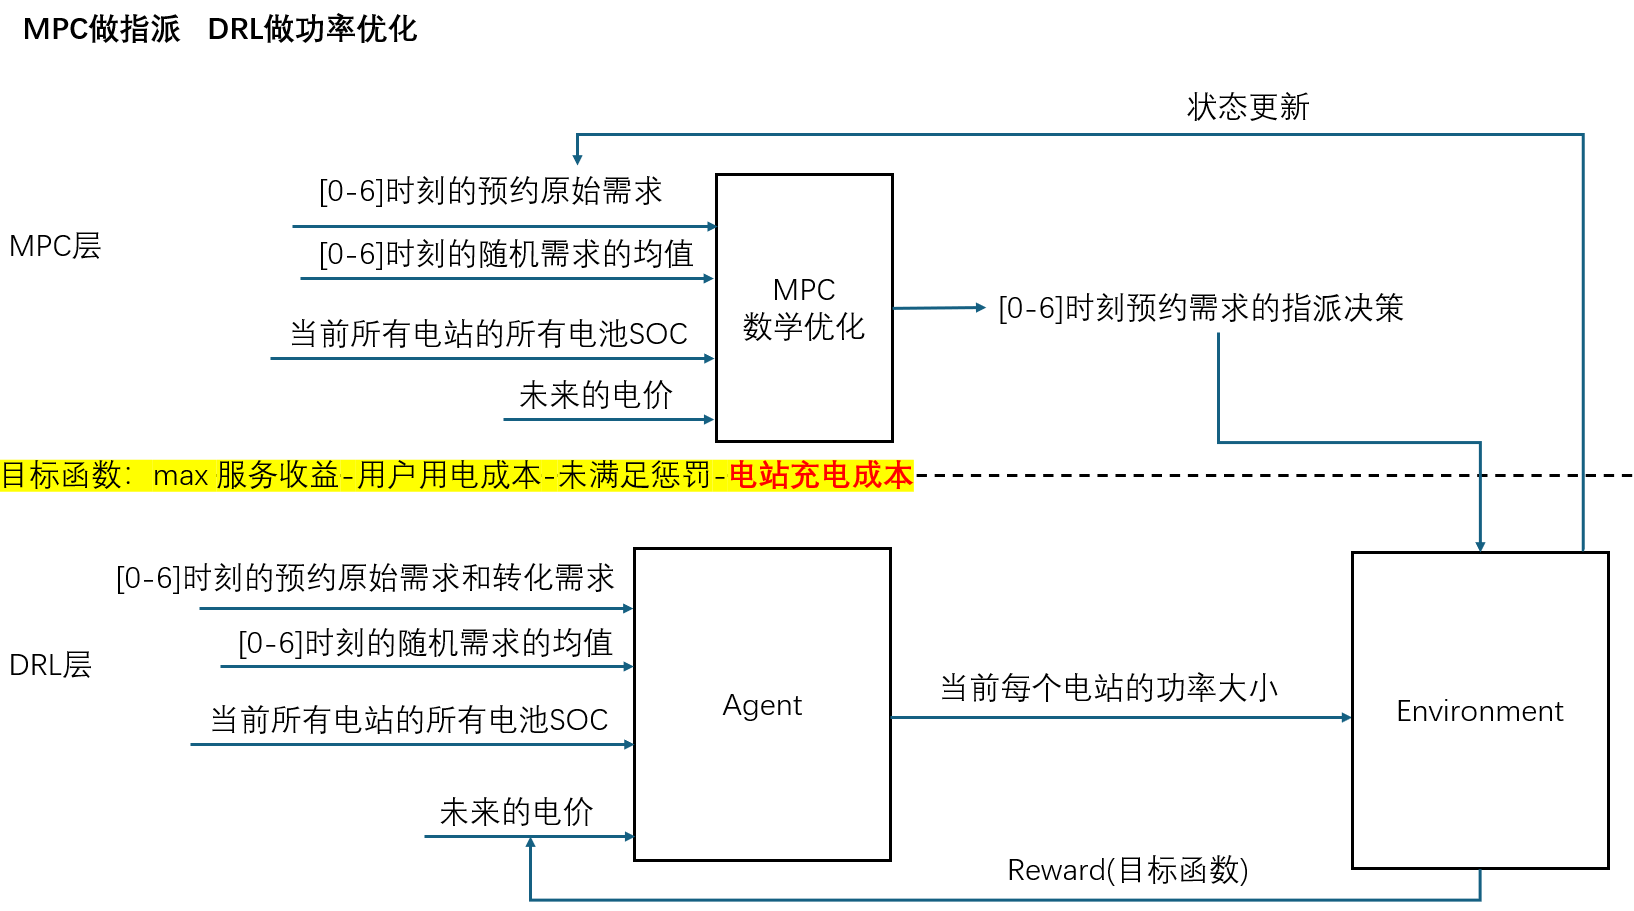
\includegraphics[width =1.0\textwidth]{figures/MPC-RL.png}
    \caption{MPC-RL协同优化框架}
    \label{fig:MPC-RL}
\end{figure}

\section{MPC Formulation}
\subsection{时域设置}

\begin{figure}[!htbp]
    \centering
    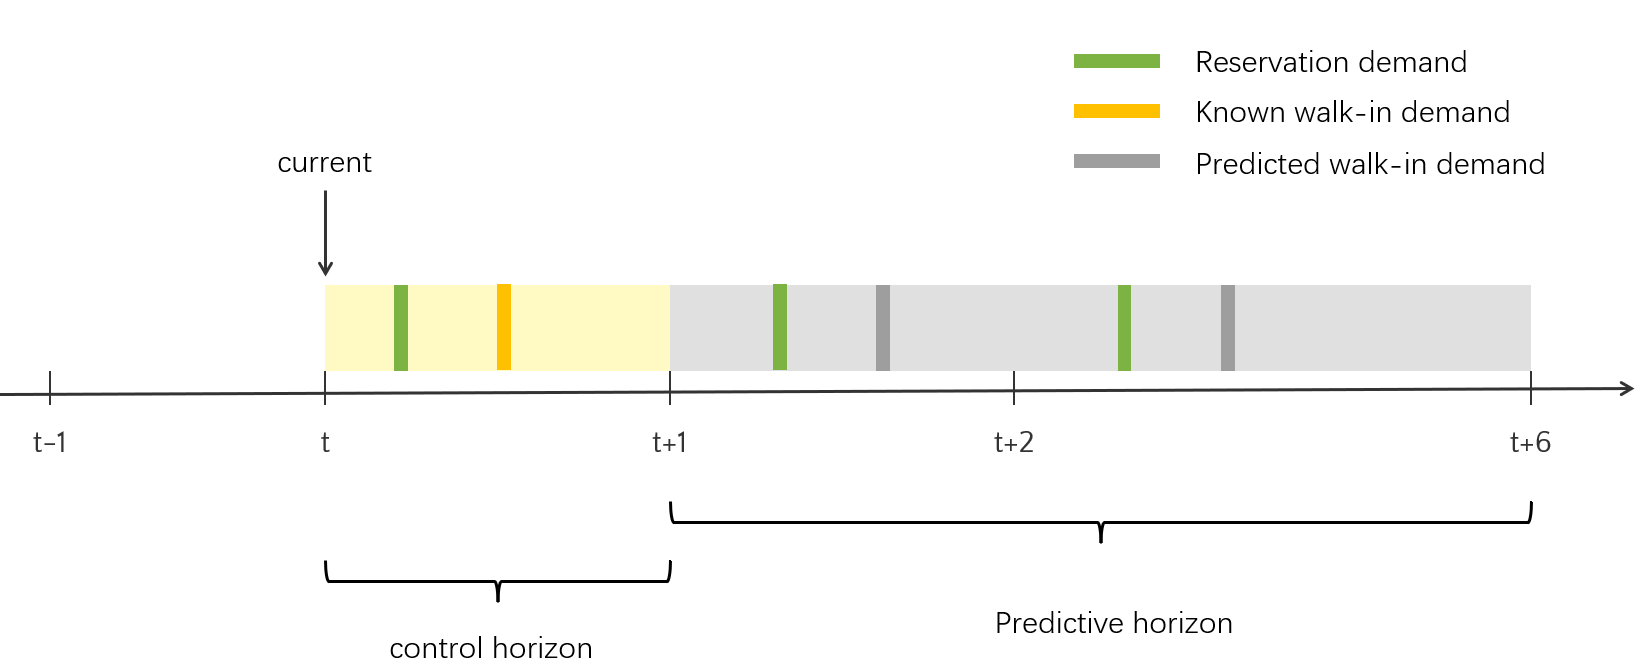
\includegraphics[width =1.0\textwidth]{figures/time_line.png}
    \caption{Rolling Horizon}
    \label{fig:Rolling Horizon}
\end{figure}

本文采用滚动时域思想刻画换电站运营中的动态决策过程。设当前滚动决策时刻为 $\ell$。为避免预约用户出发时段与实际换电时段之间存在旅行时间滞后而造成预测域边界问题，本文区分预约指派决策域和库存预测域。具体而言，令预约指派决策域长度为 $H^A$，库存预测域长度为 $H^w$，并定义
\begin{equation}
\mathcal{T}^{A}=\{1,\ldots,H^A\},\qquad
\mathcal{T}=\{1,\ldots,H^w\},\qquad
\mathcal{T}^{w}=\{0,1,\ldots,H^w\}.
\label{eq:horizon_sets}
\end{equation}
其中，$\mathcal{T}^{A}$ 用于预约用户的出发或指派决策，$\mathcal{T}$ 用于随机用户服务、充电过程和库存状态转移，$\mathcal{T}^{w}$ 用于刻画库存状态时点。记
\begin{equation}
\tau_{\max}=\max_{p\in\mathcal{P},\,i\in\mathcal{S}^{p}}\tau_{p,i}.
\label{eq:tau_max}
\end{equation}
本文要求
\begin{equation}
H^A+\tau_{\max}\le H^w,
\label{eq:horizon_condition}
\end{equation}
从而保证任一在当前 MPC 中被指派的预约用户，其实际到达换电站并消耗满电电池的时段均落在库存预测域内。

在每一轮 MPC 中，系统根据当前观测到的电池 SOC 库存、已知预约需求、随机需求预测、电价信息以及 RL 层给定的充电功率策略，求解库存预测域内的用户服务分配问题。求解完成后，仅执行当前时段的决策，并在进入下一时刻后根据新的系统状态重新构造并求解 MPC 问题。预约用户服务变量 $y_{A,i,j}^{n,p,t}$ 仅定义在 $t\in\mathcal{T}^{A}$ 上；随机用户服务变量 $y_R^{n,i,t}$ 定义在 $t\in\mathcal{T}$ 上；电池库存变量 $w_{n,i,t}$ 定义在状态时点 $t\in\mathcal{T}^{w}$ 上。对于预约用户，$t$ 表示其出发或指派时段，换电服务发生在其到达相应换电站的时段。本文假设旅行时间不随出发时段变化，因此 O-D 对 $p$ 的用户到达节点 $i$ 的时段为 $t+\tau_{p,i}$。预约用户的决策索引仍为出发时段 $t$，而电池消耗和状态转移通过 $t+\tau_{p,i}$ 关联到实际到达时段。由于式\eqref{eq:horizon_condition} 成立，当前 MPC 中所有被指派预约用户的换电事件均由库存转移和满电电池容量约束显式覆盖；已经在当前滚动时刻前出发但在当前库存预测域内到达的预约用户，则作为历史承诺 $\bar{y}_{A,i,j}^{n,p,k}$ 进入状态转移。

在预约用户服务方面，本文不强制要求所有预约需求均被服务，而是采用“未满足预约需求惩罚 + 预约服务率约束”的方式刻画预约用户相对于随机用户的较高服务优先级。服务率考核仅针对当前预约指派决策域 $\mathcal{T}^{A}$ 内的预约需求，而不将尚未进入本轮可指派集合的远期预约需求计入分母；这些远期需求会随着滚动时域推进，在后续 MPC 中进入新的预约指派决策域。具体而言，目标函数中引入未满足预约需求惩罚系数 $\alpha$，用于表示运营商因未服务预约用户而承担的用户补偿、信誉损失或服务质量损失；同时设置预约服务率下界 $\eta$，要求预约指派决策域内预约用户服务量不低于给定比例。该处理方式避免了字典序优化过于强硬的问题，也便于在数值实验中分析 $\alpha$ 和 $\eta$ 对预约服务率、随机用户服务量和系统经济收益的影响。若实际运营中要求所有成功预约用户必须得到服务，则可在后续扩展中引入预约接受控制机制。

\subsection{变量列表}

本文使用的变量如\autoref{tab:notation}所示。该符号表仅列出 MPC 优化模型所需集合、参数和决策变量；RL formulation 中的状态、动作、奖励和算法符号将在第 3 节单独定义。

\begin{table}[!htbp]
  \centering
  \caption{Notation table for the MPC optimization model}
  \label{tab:notation}
  \footnotesize
  \setlength{\tabcolsep}{2pt}
  \renewcommand{\arraystretch}{0.88}
  \begin{tabular}{@{}lp{13cm}@{}}
    \toprule
    \textbf{Notation} & \textbf{Description} \\
    \midrule
    \multicolumn{2}{l}{\textit{Sets and Indices}} \\
    $\mathcal{P}$ & Set of O-D pairs, indexed by $p$ \\
    $\mathcal{T}^{A}$ & Set of reservation assignment periods, $\mathcal{T}^{A}:=\{1,\dots,H^A\}$, indexed by $t$ or $k$ \\
    $\mathcal{T}$ & Set of operational periods in the inventory prediction horizon, $\mathcal{T}:=\{1,\dots,H^w\}$, indexed by $t$ \\
    $\mathcal{T}^{w}$ & Set of battery inventory state points, $\mathcal{T}^{w}:=\{0,1,\dots,H^w\}$ \\
    $\mathcal{N}$ & Set of discretized battery SOC states, $\mathcal{N}:=\{0,\dots,N\}$, indexed by $n,m,r$ \\
    $\mathcal{S}^{p}$ & Set of intermediate BSSs on the path of O-D pair $p$, indexed by $i,j$ \\
    $\mathcal{S}$ & Set of all BSSs in the system, $\mathcal{S}:=\bigcup_{p\in\mathcal{P}}\mathcal{S}^{p}$ \\
    $\mathcal{V}^{p}$ & Node set consisting of origin $o^{p}$, destination $d^{p}$, and BSSs $\mathcal{S}^{p}$ on the path of O-D pair $p$ \\
    $\mathcal{A}^{n,p}$ & Arc set in the SOC-wise expanded network for initial SOC state $n$ and O-D pair $p$ \\
    $\mathcal{G}^{n,p}$ & Directed graph for initial SOC state $n$ and O-D pair $p$, $\mathcal{G}^{n,p}:=(\mathcal{V}^{p},\mathcal{A}^{n,p})$ \\
    \midrule
    \multicolumn{2}{l}{\textit{Parameters}} \\
    $H^A$ & Length of the reservation assignment horizon \\
    $H^w$ & Length of the inventory prediction horizon \\
    $\tau_{p,i}$ & Travel time from the origin to node $i$ for an EV of O-D pair $p$; it is independent of the departure time \\
    $\tau_{p,\max}$ & Maximum travel time of EVs for O-D pair $p$ \\
    $\tau_{\max}$ & Maximum travel time over all O-D pairs and BSSs, $\tau_{\max}:=\max_{p\in\mathcal{P},\,i\in\mathcal{S}^{p}}\tau_{p,i}$; the horizons satisfy $H^A+\tau_{\max}\le H^w$ \\
    $P_{n,i,t}$ & Charging increment or power applied to batteries with SOC state $n$ at station $i$ during period $t$; it is provided by the RL layer and treated as a parameter in MPC \\
    $e_{i,t}$ & Electricity price at station $i$ during period $t$ \\
    $s$ & Fixed unit swapping service fee, independent of station and time \\
    $v^{p}_{i,j}$ & Energy consumption from node $i$ to node $j$ for an EV of O-D pair $p$; it is independent of the user's initial SOC \\
    $\alpha$ & Penalty cost per unit of unsatisfied reservation demand \\
    $\eta$ & Minimum reservation service rate required within the reservation assignment horizon \\
    $\beta$ & Weight coefficient of the RL-enhanced terminal value in the MPC objective \\
    $\lambda_{i,n,\ell}$ & Marginal terminal value of one additional battery with SOC state $n$ at station $i$ at the current rolling decision epoch $\ell$ \\
    $f_{A}^{n,p,t}$ & Reservation demand volume of EVs with initial SOC state $n$ for O-D pair $p$ departing in period $t\in\mathcal{T}^{A}$ \\
    $f_{R}^{n,i,t}$ & Random demand volume of EVs with returned SOC state $n$ at station $i$ in period $t$ \\
    $\bar{y}_{A,i,j}^{n,p,k}$ & Historical service volume of reservation flows on arc $(i,j)$ that departed before the current rolling epoch, $k\in\{-\tau_{p,\max},\dots,0\}$ \\
    $\bar{w}_{n,i,0}$ & Initial number of batteries with SOC state $n$ at station $i$ at the beginning of the inventory prediction horizon \\
    $\underline{w}_{N,i}$ & Minimum number of fully charged batteries retained at station $i$ at the terminal inventory state \\
    $\Phi^{\mathrm{RL}}_{\ell}$ & Linear terminal value term provided by the RL critic at the current rolling decision epoch $\ell$, evaluated at the terminal inventory state $H^w$ \\
    \midrule
    \multicolumn{2}{l}{\textit{Decision Variables}} \\
    $y_{A,i,j}^{n,p,t}$ & Service flow of reservation demand $f_{A}^{n,p,t}$ on arc $(i,j)\in\mathcal{A}^{n,p}$, defined for $t\in\mathcal{T}^{A}$ \\
    $y_{R}^{n,i,t}$ & Service volume of random demand $f_{R}^{n,i,t}$ at station $i$ in period $t\in\mathcal{T}$ \\
    $w_{n,i,t}$ & Number of batteries with SOC state $n$ at station $i$ at inventory state point $t\in\mathcal{T}^{w}$ \\
    \bottomrule
  \end{tabular}
\end{table}

\subsection{SOC-wise expanded network}

高速公路换电场景中的预约用户具有明确的 OD 路径和初始 SOC。由于初始 SOC 不同，同一 OD 对上的用户可达站点集合和可行换电路径可能不同。为刻画这种 SOC 相关的路径可行性，本文在传统 expanded network 的基础上构建 SOC-wise expanded network。该建模方法针对每一个 OD 对 $p\in\mathcal{P}$ 和每一个初始 SOC 状态 $n\in\mathcal{N}$，分别构造一个有向网络 $\mathcal{G}^{n,p}=(\mathcal{V}^{p},\mathcal{A}^{n,p})$。

在网络 $\mathcal{G}^{n,p}$ 中，节点集合 $\mathcal{V}^{p}$ 包括 OD 对 $p$ 的起点 $o^p$、终点 $d^p$ 以及该路径上可经过的所有中间换电站 $\mathcal{S}^{p}$。弧集合 $\mathcal{A}^{n,p}$ 用于表示在初始 SOC 为 $n$ 的条件下，用户从一个节点行驶到另一个节点并完成后续换电服务的可行连接。弧的可行性由路段能耗 $v^p_{i,j}$ 与车辆可用电量共同决定：若弧从起点 $o^p$ 出发，则要求 $n\ge v^p_{o^p,j}$；若弧从某一中间换电站出发，则车辆刚完成换电并获得满电电池，因而要求 $N\ge v^p_{i,j}$。因此，能耗参数 $v^p_{i,j}$ 本身不需要索引初始 SOC，而初始 SOC 的影响通过网络弧集合 $\mathcal{A}^{n,p}$ 体现。

该网络建模方式具有两个作用。第一，它将用户初始 SOC 对可达站点和换电路径的影响显式嵌入网络结构，使得不可行的站点选择不会进入优化模型。第二，它使预约用户指派问题可以表示为网络流决策：预约指派决策域内的预约需求 $f_A^{n,p,t}$ 从起点 $o^p$ 进入网络，服务变量 $y_{A,i,j}^{n,p,t}$ 表示该类需求在弧 $(i,j)\in\mathcal{A}^{n,p}$ 上的服务流量，其中 $t\in\mathcal{T}^{A}$。通过流平衡约束，模型可以保证被服务的预约用户沿一条可行路径从起点移动到终点，并在路径上的换电站消耗满电电池、归还低 SOC 电池。

需要注意的是，SOC-wise expanded network 主要用于刻画预约用户的可行路径和站点指派。随机用户由于在换电站现场到达，本文不再为其构造 OD 网络，而是直接通过 $y_R^{n,i,t}$ 表示时段 $t$、站点 $i$、退回 SOC 为 $n$ 的随机用户服务量。预约用户和随机用户在电池库存层面相互耦合：两类用户服务均会消耗站内满电电池，并向站内归还不同 SOC 状态的电池。

\begin{figure}[!htbp]
    \centering
    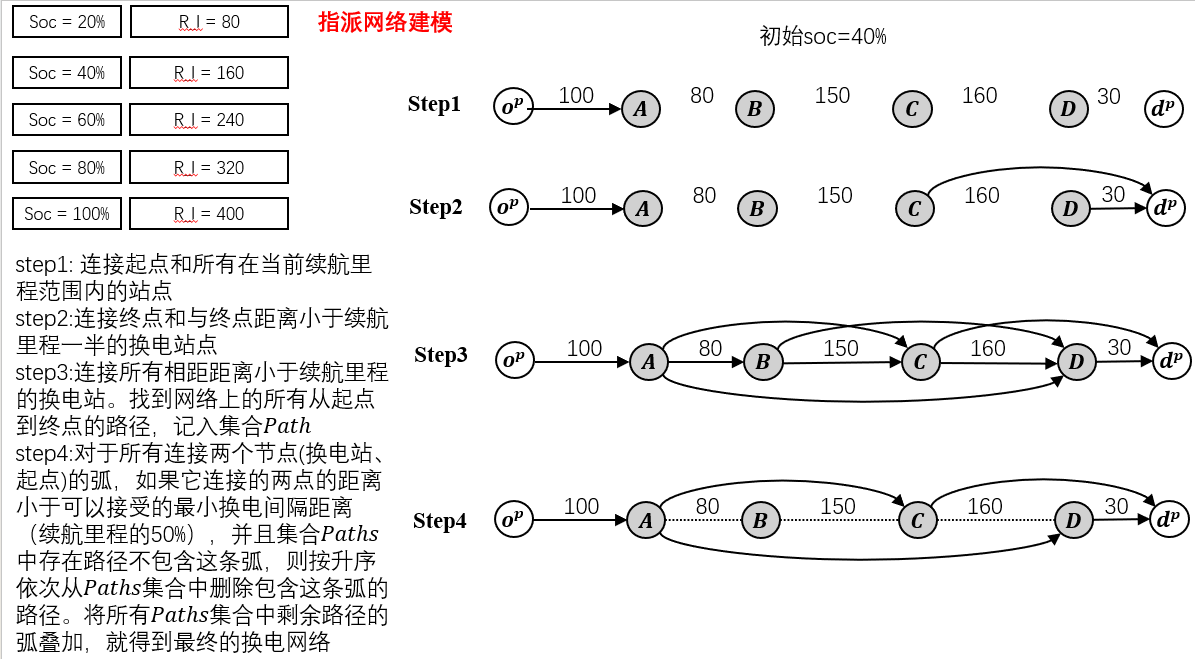
\includegraphics[width =1.0\textwidth]{figures/指派网络建模.png}
    \caption{指派网络建模}
    \label{fig:assignment network}
\end{figure}

\subsection{Mathematical model}

本节给出 MPC 层的数学规划模型。MPC 层的决策变量包括预约用户在 SOC-wise expanded network 上的服务流量 $y_{A,i,j}^{n,p,t}$、随机用户服务量 $y_R^{n,i,t}$ 以及各站点不同 SOC 电池库存 $w_{n,i,t}$。其中，预约指派变量定义在 $t\in\mathcal{T}^{A}$ 上，随机用户服务变量和库存转移定义在 $t\in\mathcal{T}$ 上。RL 层输出的充电功率 $P_{n,i,t}$ 在每轮 MPC 求解时作为外部给定参数进入电池状态转移和充电成本项。与前文设定一致，服务费为固定单位服务费 $s$，旅行时间为只依赖于 O-D 对和到达节点的参数 $\tau_{p,i}$。

为刻画预约用户到达站点后的退回电池 SOC，定义辅助函数
\begin{equation}
\rho_{j,i}^{n,p}=
\begin{cases}
 n-v_{j,i}^{p}, & j=o^p,\\
 N-v_{j,i}^{p}, & j\in\mathcal{S}^{p},
\end{cases}
\label{eq:return_soc}
\end{equation}
其中 $\rho_{j,i}^{n,p}$ 表示初始 SOC 为 $n$ 的预约用户沿弧 $(j,i)$ 到达站点 $i$ 时退回电池的 SOC。第一种情况对应用户从起点携带原始电池行驶至第一个换电站，第二种情况对应用户在前一换电站换得满电电池后继续行驶。

为简化表达，定义时段 $t$ 站点 $i$ 需要消耗满电电池的当前预约服务量和历史预约服务量分别为
\begin{align}
Q_{i,t}^{A,\mathrm{cur}}
&=
\sum_{p\in\mathcal{P}}
\sum_{n\in\mathcal{N}}
\sum_{\{j\mid (j,i)\in\mathcal{A}^{n,p}\}}
\sum_{\{k\in\mathcal{T}^{A}\mid k+\tau_{p,i}=t\}}
y_{A,j,i}^{n,p,k},
\label{eq:current_reservation_swap}\\
Q_{i,t}^{A,\mathrm{his}}
&=
\sum_{p\in\mathcal{P}}
\sum_{n\in\mathcal{N}}
\sum_{\{j\mid (j,i)\in\mathcal{A}^{n,p}\}}
\sum_{\{k\in\{-\tau_{p,\max},\ldots,0\}\mid k+\tau_{p,i}=t\}}
\bar{y}_{A,j,i}^{n,p,k}.
\label{eq:historical_reservation_swap}
\end{align}
上述两个量均采用到达站点 $i$ 的入弧流量，因为电池在用户到达站点 $i$ 并完成换电时被消耗。

有限库存预测域 MPC 若仅优化库存预测域内收益，可能在时域末端过度服务当前用户，从而留下对未来运营不利的库存结构。为缓解这一末端效应，本文利用 RL critic 学到的长期价值信息构造线性终端价值项。RL critic 学习状态价值函数
\begin{equation}
V_{\theta}(s_t)\approx
\mathbb{E}\left[\sum_{h=0}^{\infty}\gamma^h r_{t+h}\mid s_t\right].
\label{eq:critic_value}
\end{equation}
由于 $V_{\theta}(s)$ 通常由深度神经网络表示，直接将其嵌入 MPC 会导致优化模型非线性且难以求解。因此，本文仅利用 critic 提取终端库存的局部边际价值。在每轮 MPC 求解前，先构造参考终端状态 $\bar{s}_{\ell+H^w}$，然后在该状态处对 $V_{\theta}(s)$ 关于终端库存进行一阶线性化：
\begin{equation}
V_{\theta}(s_{\ell+H^w})
\approx
V_{\theta}(\bar{s}_{\ell+H^w})+
\sum_{i\in\mathcal{S}}\sum_{n\in\mathcal{N}}
\lambda_{i,n,\ell}\left(w_{n,i,H^w}-\bar{w}_{n,i,H^w}\right),
\label{eq:value_linearization}
\end{equation}
其中
\begin{equation}
\lambda_{i,n,\ell}
=
\left.
\frac{\partial V_{\theta}(s)}{\partial w_{n,i}}
\right|_{s=\bar{s}_{\ell+H^w}},
\quad \forall i\in\mathcal{S},\ n\in\mathcal{N}.
\label{eq:marginal_value}
\end{equation}
常数项不影响 MPC 最优解，因此目标函数中仅保留线性终端价值项
\begin{equation}
\Phi^{\mathrm{RL}}_{\ell}
=
\sum_{i\in\mathcal{S}}\sum_{n\in\mathcal{N}}
\lambda_{i,n,\ell}w_{n,i,H^w}.
\label{eq:rl_terminal_value}
\end{equation}
在 MPC 求解时，$\lambda_{i,n,\ell}$ 是固定参数，故式\eqref{eq:rl_terminal_value} 对库存变量保持线性，不会破坏原优化模型的可求解性。


\subsubsection{Reservation service priority representation}

本文不采用字典序优化，而是通过未满足预约需求惩罚和预约服务率约束共同刻画预约用户的较高服务优先级。由于预约用户的换电事件发生在出发时段之后，为避免服务率约束将本轮尚不能完整决策和约束的远期预约需求纳入分母，本文仅在预约指派决策域 $\mathcal{T}^{A}$ 内计算预约服务率。首先定义预约指派决策域内被服务的预约需求总量：
\begin{equation}
S_A^{\mathrm{dec}}(y_A)=
\sum_{t\in\mathcal{T}^{A}}\sum_{p\in\mathcal{P}}\sum_{n\in\mathcal{N}}
\sum_{\{j\mid (o^p,j)\in\mathcal{A}^{n,p}\}}
y_{A,o^p,j}^{n,p,t}.
\label{eq:served_reservation_total}
\end{equation}
预约指派决策域内预约需求总量为
\begin{equation}
D_A^{\mathrm{dec}}=
\sum_{t\in\mathcal{T}^{A}}\sum_{p\in\mathcal{P}}\sum_{n\in\mathcal{N}}
f_A^{n,p,t}.
\label{eq:reservation_total_demand}
\end{equation}
因此，未满足预约需求量可表示为 $U_A^{\mathrm{dec}}=D_A^{\mathrm{dec}}-S_A^{\mathrm{dec}}(y_A)$，其对应的惩罚项进入目标函数。除此之外，本文设置预约服务率约束 $S_A^{\mathrm{dec}}(y_A)\ge \eta D_A^{\mathrm{dec}}$，从而保证当前可指派预约集合的服务质量最低水平。

该建模方式的含义是：预约用户并非被建模为绝对优先的刚性服务对象，而是具有更高的运营损失权重和最低服务水平保障。服务率分母仅包括当前预约指派决策域 $\mathcal{T}^{A}$ 内的预约需求；超出该决策域的远期预约需求不会被视为本轮未服务需求，而是在后续滚动时域中进入新的预约指派决策域后再参与服务率约束和未满足惩罚。参数 $\alpha$ 反映运营商对预约违约成本的重视程度，参数 $\eta$ 反映平台对预约服务质量的最低要求。通过改变 $\alpha$ 和 $\eta$，可以在数值实验中分析预约服务率、随机用户服务量和系统经济收益之间的权衡关系。

\subsubsection{Objective function}

目标函数为最大化库存预测域内的服务收益，减去未满足预约需求惩罚和电站充电成本，并加入 RL critic 提供的线性终端价值：
\begin{equation}
\max \quad I-C_1-C_2+\beta\Phi^{\mathrm{RL}}_{\ell}.
\label{eq:objective}
\end{equation}

服务收益由预约用户和随机用户完成换电所产生的服务费构成。为保持与预约指派决策的时间逻辑一致，预约用户收益项以预约指派决策域 $\mathcal{T}^{A}$ 内的出发或指派时段 $t$ 为决策索引；由于服务费为固定值，收益项不再依赖站点或到达时段：
\begin{equation}
\begin{aligned}
I=&
\sum_{t\in\mathcal{T}^{A}}\sum_{p\in\mathcal{P}}\sum_{n\in\mathcal{N}}
\sum_{i\in\mathcal{S}^{p}}
\sum_{\{j\mid (j,i)\in\mathcal{A}^{n,p}\}}
 y_{A,j,i}^{n,p,t}
\left(N-\rho_{j,i}^{n,p}\right)s
\\
&+
\sum_{t\in\mathcal{T}}\sum_{i\in\mathcal{S}}\sum_{n\in\mathcal{N}}
y_R^{n,i,t}(N-n)s.
\end{aligned}
\label{eq:income}
\end{equation}
其中 $N-\rho_{j,i}^{n,p}$ 和 $N-n$ 分别表示预约用户与随机用户在换电时获得的补能量，$s$ 为固定单位服务费。若服务费按次收取而非按补能量收取，可将上述补能量系数并入固定服务费参数中。由于 $s$ 不随站点和时间变化，收益函数中不再需要预测未来服务价格。式\eqref{eq:horizon_condition} 保证当前 MPC 中被指派预约用户的换电事件均落在库存预测域内；预测域开始前已经出发且在当前库存预测域内到达的换电服务则通过历史承诺变量进入库存转移。

未满足预约需求惩罚为
\begin{equation}
C_1 = \alpha \left(D_A^{\mathrm{dec}}-S_A^{\mathrm{dec}}(y_A)\right)
=\alpha \sum_{t\in \mathcal{T}^{A}} \sum_{p\in \mathcal{P}}  \sum_{n\in \mathcal{N}} 
\left[
f_A^{n,p,t} - \sum_{\{j \mid (o^p,j) \in \mathcal{A}^{n,p}\}} y_{A,o^p,j}^{n,p,t} \right].
\label{eq:penaltycost}
\end{equation}

电站充电成本按照时段开始时的库存和该时段的充电功率计算：
\begin{equation}
C_2 = \sum_{t \in \mathcal{T}}  \sum_{n \in \mathcal{N}} \sum_{i \in \mathcal{S}}
 w_{n,i,t-1}P_{n,i,t}e_{i,t}.
\label{eq:chargingcost}
\end{equation}

\subsubsection{Constraints}

\paragraph{Flow conservation constraints.}
预约需求从起点进入 SOC-wise expanded network，且服务量不超过实际预约需求：
\begin{subequations}
\label{eq:flow}
\begin{gather}
\sum_{\{j\mid (o^p,j)\in \mathcal{A}^{n,p}\}}{y_{A,o^p,j}^{n,p,t}} \leq f_A^{n,p,t},
\quad \forall p\in \mathcal{P},\ t\in \mathcal{T}^{A},\ n \in \mathcal{N},\label{eq:flow1}\\
\sum_{\{j\mid (i,j)\in \mathcal{A}^{n,p}\}}{y_{A,i,j}^{n,p,t}} =
\sum_{\{j\mid (j,i)\in \mathcal{A}^{n,p}\}}{y_{A,j,i}^{n,p,t}},
\quad \forall p\in \mathcal{P},\ t\in \mathcal{T}^{A},\ i\in \mathcal{S}^p,
\ n\in\mathcal{N}.
\label{eq:flow2}
\end{gather}
\end{subequations}
由于高速公路路径具有方向性，网络 $\mathcal{G}^{n,p}$ 可按路径顺序构造为无回路网络；在该条件下，起点流量结合中间站点流平衡即可保证被服务预约流最终到达终点。

\paragraph{Reservation service-level constraint.}
为保证预约用户具有高于随机用户的服务保障，本文要求预约指派决策域内预约用户服务率不低于给定阈值 $\eta$：
\begin{equation}
S_A^{\mathrm{dec}}(y_A)\ge \eta D_A^{\mathrm{dec}}.
\label{eq:reservation_service_rate}
\end{equation}
其中，$S_A^{\mathrm{dec}}(y_A)$ 和 $D_A^{\mathrm{dec}}$ 分别由式\eqref{eq:served_reservation_total} 和式\eqref{eq:reservation_total_demand} 定义。当 $\eta$ 趋近于 1 时，模型更接近对预约用户的刚性服务保障；当 $\eta$ 较低时，模型具有更大的经济优化自由度。该约束与目标函数中的未满足预约惩罚共同体现预约用户的较高服务优先级。由于 $D_A^{\mathrm{dec}}$ 不包含超出预约指派决策域的远期预约需求，服务率约束不会因为本轮未决策的预约需求而被人为拉低。

\paragraph{Battery state transition constraints.}
为表示充电导致的 SOC 转移，定义
\begin{equation}
\chi_{m,i,t}^{r}=\mathbb{I}\!\left(\min\{m+P_{m,i,t},N\}=r\right),
\quad \forall m,r\in\mathcal{N},\ i\in\mathcal{S},\ t\in\mathcal{T}.
\label{eq:charging_indicator}
\end{equation}
若 SOC 和功率均采用离散刻度，$\chi_{m,i,t}^{r}$ 表示时点 $t-1$ 处于 SOC $m$ 的电池经过时段 $t$ 的充电后，在时点 $t$ 转移至 SOC $r$。

对于 SOC 状态 $r<N$ 的电池，时点 $t$、站点 $i$ 的库存由当前库存预测域内到达并归还 SOC 为 $r$ 电池的预约用户、当前滚动时刻前已经出发但在当前库存预测域内到达的历史预约用户、当前随机用户归还的 SOC 为 $r$ 电池，以及上一时点经过充电后转移到 SOC $r$ 的站内电池构成：
\begin{equation}
\begin{aligned}
w_{r,i,t}
=&
\sum_{p\in \mathcal{P}}
\sum_{n\in \mathcal{N}}
\sum_{\{j\mid (j,i)\in \mathcal{A}^{n,p}\}}
\sum_{\{k\in \mathcal{T}^{A}\mid k+\tau_{p,i}=t\}}
y_{A,j,i}^{n,p,k}
\mathbb{I}\!\left(\rho_{j,i}^{n,p}=r\right)
\\
&+
\sum_{p\in \mathcal{P}}
\sum_{n\in \mathcal{N}}
\sum_{\{j\mid (j,i)\in \mathcal{A}^{n,p}\}}
\sum_{\{k\in\{-\tau_{p,\max},\ldots,0\}\mid k+\tau_{p,i}=t\}}
\bar{y}_{A,j,i}^{n,p,k}
\mathbb{I}\!\left(\rho_{j,i}^{n,p}=r\right)
\\
&+
y_R^{r,i,t}
+
\sum_{m\in \mathcal{N}}
w_{m,i,t-1}\chi_{m,i,t}^{r},
\\
&\forall i\in \mathcal{S},\ r\in \mathcal{N}\setminus\{N\},\ t\in \mathcal{T}.
\end{aligned}
\label{eq:transition_nonfull}
\end{equation}

对于满电电池，时点 $t$ 的库存等于上一时点经过充电达到满电的电池数量，减去当前时段被预约用户和随机用户换走的满电电池数量：
\begin{equation}
\begin{aligned}
w_{N,i,t}
=&
\sum_{m\in \mathcal{N}}
w_{m,i,t-1}\chi_{m,i,t}^{N}
-
Q_{i,t}^{A,\mathrm{cur}}
-
Q_{i,t}^{A,\mathrm{his}}
-
\sum_{n\in \mathcal{N}}y_R^{n,i,t},
\\
&\forall i\in \mathcal{S},\ t\in \mathcal{T}.
\end{aligned}
\label{eq:transition_full}
\end{equation}


\paragraph{Swapping capacity constraints.}
令时段 $t$ 站点 $i$ 在服务用户前可用于换电的满电电池数量为
\begin{equation}
F_{i,t}=\sum_{m\in\mathcal{N}}w_{m,i,t-1}\chi_{m,i,t}^{N}.
\label{eq:available_full_batteries}
\end{equation}
则预约用户和随机用户的总换电服务量不能超过可用满电电池数量：
\begin{equation}
Q_{i,t}^{A,\mathrm{cur}}+Q_{i,t}^{A,\mathrm{his}}+
\sum_{n\in\mathcal{N}}y_R^{n,i,t}
\le F_{i,t},
\quad \forall i\in\mathcal{S},\ t\in\mathcal{T}.
\label{eq:full_battery_capacity}
\end{equation}
该约束刻画预约用户和随机用户对满电电池资源的共同容量限制。不同于字典序优化或局部剩余容量规则，本文通过式\eqref{eq:reservation_service_rate} 的服务率下界和式\eqref{eq:penaltycost} 的未满足预约惩罚来体现预约用户的软优先级；式\eqref{eq:full_battery_capacity} 本身仅负责保证物理可行性，即总换电服务量不能超过满电电池供给量。

随机用户服务量不得超过实际随机需求：
\begin{equation}
0\le y_R^{n,i,t}\le f_R^{n,i,t},
\qquad
\forall i\in \mathcal{S},\ n\in \mathcal{N},\ t\in \mathcal{T}.
\label{eq:random_bound}
\end{equation}

\paragraph{Boundary and integrality constraints.}
库存预测域起点的电池 SOC 分布为已知初始状态：
\begin{equation}
w_{n,i,0}=\bar{w}_{n,i,0},
\quad \forall n\in \mathcal{N},\ i\in \mathcal{S}.
\label{eq:initial_inventory}
\end{equation}

所有服务量和电池库存变量均应满足非负性约束：
\begin{gather}
w_{n,i,t}\ge 0,
\quad \forall n\in \mathcal{N},\ i\in \mathcal{S},\ t\in \mathcal{T}^{w},
\label{eq:nonnegative_w}\\
y_{A,i,j}^{n,p,t}\ge 0,
\quad \forall p\in \mathcal{P},\ n\in \mathcal{N},\ t\in \mathcal{T}^{A},\ (i,j)\in \mathcal{A}^{n,p},
\label{eq:nonnegative_a}\\
y_R^{n,i,t}\ge 0,
\quad \forall n\in \mathcal{N},\ i\in \mathcal{S},\ t\in \mathcal{T}.
\label{eq:nonnegative_r}
\end{gather}

若需求量和电池数量均以整数计，则进一步有
\begin{equation}
w_{n,i,t}\in \mathbb{Z}_{+},\quad
 y_{A,i,j}^{n,p,t}\in \mathbb{Z}_{+},\quad
 y_R^{n,i,t}\in \mathbb{Z}_{+}.
\label{eq:integer}
\end{equation}

引入 RL 终端价值后，MPC 不再仅依赖固定终端库存下界来处理末端效应。式\eqref{eq:rl_terminal_value} 通过 $\lambda_{i,n,\ell}$ 区分不同站点、不同 SOC 电池在未来运营中的长期边际价值，从而引导 MPC 在库存预测域末端保留更有价值的库存结构。与此同时，为保证运行安全，仍可保留如下终端满电电池库存下界作为可选硬约束：
\begin{equation}
w_{N,i,H^w}\ge \underline{w}_{N,i},
\quad \forall i\in \mathcal{S}.
\label{eq:terminal_inventory}
\end{equation}
其中，$\underline{w}_{N,i}$ 表示库存预测域末端电站 $i$ 至少需要保留的满电电池数量。在本文框架中，该约束主要作为安全库存下界，而长期影响的差异化评估由 RL critic 提供的终端价值项承担。

\section{RL Formulation}

RL 层用于学习充电功率控制策略，并通过 critic 为 MPC 提供终端库存价值信息。本节将充电功率控制问题建模为马尔可夫决策过程，并给出本文采用的 RL 算法。

\subsection{Markov decision process}

\paragraph{State.}
在决策时刻 $t$，RL agent 观测系统状态 $s_t$。状态应包含影响当前充电功率决策及其长期后果的关键信息，主要包括各站点、各 SOC 状态的电池库存，未来预约需求，随机需求预测，未来电价，以及时间特征等：
\begin{equation}
s_t=
\left(
\{w_{n,i,t}\}_{i\in\mathcal{S},n\in\mathcal{N}},
\{f_A^{n,p,\tau}\}_{\tau\in\mathcal{H}_t},
\{\hat f_R^{n,i,\tau}\}_{\tau\in\mathcal{H}_t},
\{e_{i,\tau}\}_{\tau\in\mathcal{H}_t},
\xi_t
\right),
\label{eq:rl_state}
\end{equation}
其中 $\mathcal{H}_t$ 表示 RL 可获得的预测信息窗口，$\xi_t$ 表示时段、节假日或交通高峰等外生时间特征。状态中包含未来预测信息，是因为充电功率决策对后续满电电池供给和充电成本具有跨时段影响。

\paragraph{Action.}
RL 的动作是充电功率决策。本文将动作表示为各站点、各 SOC 状态电池在当前时段采用的充电功率向量：
\begin{equation}
a_t=
\{P_{n,i,t}\}_{i\in\mathcal{S},n\in\mathcal{N}}.
\label{eq:rl_action}
\end{equation}
动作需要满足功率上下界和充电资源限制。实际执行时，可将 actor 网络输出映射到可行功率区间，并通过投影或裁剪保证 $P_{n,i,t}$ 不超过站点充电能力和充电槽数量限制。该动作随后作为参数输入 MPC 层，用于计算充电成本和电池 SOC 状态转移。

\paragraph{Transition.}
给定状态 $s_t$ 和动作 $a_t$ 后，系统首先以 $P_{n,i,t}$ 作为充电功率参数求解 MPC 用户服务分配模型，得到预约用户服务流量 $y_A$ 和随机用户服务量 $y_R$。随后，环境根据用户服务结果、随机需求实现值以及电池充电过程更新各站点 SOC 库存，并进入下一状态 $s_{t+1}$。因此，状态转移可抽象表示为
\begin{equation}
s_{t+1}\sim \mathcal{P}(\cdot\mid s_t,a_t,\mathrm{MPC}(s_t,a_t)),
\label{eq:rl_transition}
\end{equation}
其中 $\mathrm{MPC}(s_t,a_t)$ 表示在当前状态和充电功率动作下求解得到的用户服务分配决策。

\paragraph{Reward.}
RL reward 与系统运营目标保持一致，由实际执行时段内的服务收益、未满足预约需求惩罚和充电成本构成：
\begin{equation}
r_t=I_t-C_{1,t}-C_{2,t}.
\label{eq:rl_reward}
\end{equation}
其中 $I_t$、$C_{1,t}$ 和 $C_{2,t}$ 分别表示当前执行时段内实现的服务收益、未满足预约需求惩罚和充电成本。通过该 reward 设计，RL 层能够学习在不同需求、电价和库存状态下如何选择充电功率，以提高长期累计运营收益。

\subsection{RL algorithm}

由于充电功率是连续动作，且需要在不确定需求环境下保持训练稳定性，本文采用 Proximal Policy Optimization (PPO) 作为 RL 层的训练算法。PPO 属于 actor-critic 方法，actor $\pi_{\phi}(a_t\mid s_t)$ 输出连续充电功率动作的随机策略，critic $V_{\theta}(s_t)$ 估计当前状态的长期价值。选择 PPO 的一个重要原因是其 critic 直接学习 state value function，便于后续通过式\eqref{eq:marginal_value} 提取终端库存边际价值并传递给 MPC。

PPO 的 critic 通过最小化价值函数误差进行训练：
\begin{equation}
L_V(\theta)=
\mathbb{E}_t\left[
\left(V_{\theta}(s_t)-\hat{G}_t\right)^2
\right],
\label{eq:value_loss}
\end{equation}
其中 $\hat{G}_t$ 为由采样轨迹计算得到的折扣回报或 bootstrap return。actor 则采用 clipped surrogate objective 更新策略。定义重要性采样比率
\begin{equation}
\rho_t(\phi)=
\frac{\pi_{\phi}(a_t\mid s_t)}{\pi_{\phi_{old}}(a_t\mid s_t)},
\label{eq:ppo_ratio}
\end{equation}
则策略优化目标为
\begin{equation}
L_{\mathrm{CLIP}}(\phi)=
\mathbb{E}_t\left[
\min\left(
\rho_t(\phi)\hat{A}_t,
\mathrm{clip}(\rho_t(\phi),1-\epsilon,1+\epsilon)\hat{A}_t
\right)
\right],
\label{eq:ppo_clip}
\end{equation}
其中 $\hat{A}_t$ 为优势函数估计，$\epsilon$ 为 clip 参数。优势函数可由广义优势估计（Generalized Advantage Estimation, GAE）计算：
\begin{equation}
\hat{A}_t=\sum_{l=0}^{\infty}(\gamma\zeta)^l\delta_{t+l},
\quad
\delta_t=r_t+\gamma V_{\theta}(s_{t+1})-V_{\theta}(s_t),
\label{eq:gae}
\end{equation}
其中 $\zeta$ 为 GAE 参数。

训练完成后，actor 用于在每个决策时刻输出充电功率动作；critic 则用于提供 MPC 终端价值信息。具体而言，在每轮 MPC 求解前，系统构造参考终端状态 $\bar{s}_{\ell+H^w}$，并通过自动微分计算 $V_{\theta}(s)$ 关于库存输入 $w_{n,i}$ 的梯度，得到 $\lambda_{i,n,\ell}$。该系数随后作为固定参数进入 MPC 目标函数中的线性终端价值项 $\Phi_{\ell}^{\mathrm{RL}}$。由此，RL 层不仅提供充电功率控制动作，还将长期价值信息反馈给 MPC，形成闭环的 MPC-RL 协同优化机制。

\section{Experiments}

本节待补充。

\section{Conclusion}

本节待补充。

%%----------- 参考文献 -------------------%%
%在reference.bib文件中填写参考文献，此处自动生成

\reference

\end{document}
